%!TEX root = ComputerScienceOne.tex

%%Chapter: Functions in C
\index{functions!in C}
\index{C!functions}

As a procedural-style language, functions are essential in C 
programming.  As we've already seen, C provides a large
library of standard functions to perform basic input/output, 
math, and many other functions.  C also provides the ability 
to define and use your own functions.

When you define functions in C, careful thought must be 
made as to the naming of your functions.  This is because
C does \emph{not} support function overloading.  When you
name a function, that is the \emph{only} function that can
have that name.  Consequently, you cannot, in general,
use the same function names as defined in the standard 
libraries or any other 3rd party library that you would like
to use in your programs.

C supports both call by value and call by reference using
\emph{pointers} (see Section \ref{section:cPointers}).  C
also supports vararg functions (\mintinline{c}{printf()} being
a prime example) and allows you to define vararg functions, 
but we will not cover them in depth here.  Finally, 
parameters are not, in general, optional.  For modern 
versions of C the omission of parameters is a syntax error.
For older versions, complex rules dictate what happens
when arguments are omitted, but doing so usually results
in garbage.

\section{Defining \& Using Functions}

For modern C, defining functions is a two step process.  First,
you \emph{declare} a and its signature using a \emph{prototype}.  
Then you \emph{define} the
function by providing a function body that defines what the
function does.

\subsection{Declaration: Prototypes}
\index{function prototype}

Just as with variables, functions in C must be \emph{declared} before
they can be used.  The modern way to declare a function in C is to
use a \emph{prototype} declaration which specifies the function's
signature including its return type, identifier, and parameters.  However,
a prototype does \emph{not} include the actual body of function. 
Instead, the function's \emph{definition}, which includes the function body is
included later in the program.  Consequently, a prototype always 
ends with a semicolon.  

Typically, the documentation for functions is included with the prototype
but is \emph{not} repeated with the function definition.  This is a 
principle known as \gls{dryLabel}.  Consider the following examples.
In these examples we use a commenting style known as ``doc comments.''
This style was originally developed for Java but has since been 
adopted by many other languages.

\begin{minted}{c}
/**
 * Computes the sum of the two arguments.
 */
int sum(int a, int b);

/**
 * Computes the Euclidean distance between the 2-D points, 
 * (x1,y1) and (x2,y2).
 */
double getDistance(double x1, double y1, double x2, double y2);

/**
 * Computes a monthly payment for a loan with the given
 * principle at the given APR (annual percentage rate) which
 * is to be repaid over the given number of terms (usually
 * months).
 */
double getMonthlyPayment(double principle, double apr, int terms);
\end{minted}

In each of these, the return type is the first thing specified.  The 
function identifier (name) is then specified.  Function names must
follow the same naming rules as variables: they must begin with
an alphabetic character and may contain alphanumeric characters
as well as underscores.  Using modern coding conventions 
we usually name functions using lower camel casing.

Each prototype ends with a semicolon.  Further, 
prototypes do \emph{not} specify what the function does, they
only specify its signature.  Later in the program, we can provide
the actual definition of each function by using the following syntax.
We repeat the signature, but instead of using a semicolon, we provide
a code block, enclosed using opening/closing curly brackets, that
specifies the function body.  Here are the definitions from the 
prototype examples above:

\begin{minted}{c}
int sum(int a, int b) {
  return (a + b);
}

double getDistance(double x1, double y1, double x2, double y2) {
  double xDiff = (x1-x2);
  double yDiff = (y1-y2);
  return sqrt( xDiff * xDiff + yDiff * yDiff);
}

double getMonthlyPayment(double principle, double apr, int terms) {
  double rate = (apr / 12.0);
  double payment = (principle * rate) / (1-pow(1+rate, -terms));
  return payment;
}
\end{minted}

The keyword \mintinline{c}{return} is used to specify the value
that is returned to the calling function.

\subsection{Void Functions}

The keyword \mintinline{c}{void} can be used in C to indicate
a function does \emph{not} return a value, in which case it is
called a ``void function.''  Though it is not necessary, it is still
good practice to include a \mintinline{c}{return} statement.

\begin{minted}{c}
//prototype:
void printCopyright();

//definition:
void printCopyright() {
  printf("(c) Bourke 2015\n");
  return;
}
\end{minted}

In the example above, we've also illustrated how to define a 
function that has no inputs.  Some sources may include an 
explicit \mintinline{c}{void} keyword as a parameter to indicate
the function takes no parameters as in \mintinline{c}{void printCopyright(void);}.

\subsection{Organizing Functions}

The separation of a function declaration (prototype) and a function definition
provides a natural way to organize functions in C.  We place 
prototypes into a \emph{header} file which has a file extension
\mintinline{text}{.h} and then place the corresponding function
definitions into a \emph{source} file with the file extension, 
\mintinline{text}{.c}.

We've seen this before with the standard libraries: we use
\mintinline{c}{#include<math.h>} to ``include'' the math library's
header file in our code.  This essentially brings in the math
library function prototypes so that we can write calls to functions
like 
\mintinline{c}{sqrt()} or \mintinline{c}{sin()}.  Only when we compile 
do we actually need to \emph{link} our code to the function definitions.

When we separate prototypes into header files and definitions into
source files we also need to ``include'' the prototypes in our source file
just as we would need to include them in any other file in which we
use one of the functions.  Suppose our functions above have their
prototypes in a file named \mintinline{text}{utils.h} and their definitions
in a file named \mintinline{text}{utils.c}.  In the \mintinline{text}{utils.c}
source file we would typically use the following syntax to include
the header file:

\mintinline{c}{#include "utils.h"}

We use the double quote syntax with user-defined libraries while the
usual less-than/greater-than syntax is used with standard libraries.
With the less-than/greater-than syntax, the compiler will  
attempt to look for the header file(s) in a specified system directory
which it will fail to find if it is a user-defined library.
Furthermore, other elements are usually included in header files
such as preprocessor directives and other declarations (such as
enumerated types and structures which we introduce later).

\subsection{Calling Functions}

Once a function has been defined, or at least a prototype has
been brought into scope via an \mintinline{c}{#include} statement, 
you can write code to call your function(s).  The syntax for
doing so it to simply provide the function name followed by 
parentheses containing values or variables to pass to the function.
Some examples:

\begin{minted}{c}
int a = 10, b = 20;
int c = sum(a, b); //c contains the value 30

//invoke a function with literal values:
double dist = getDistance(0.0, 0.0, 10.0, 20.0);

//invoke a function with a combination:
double p = 1500.0;
double r = 0.05;
double monthlyPayment = getMonthlyPayment(p, r, 60);
\end{minted}

By default, all primitive types including \mintinline{c}{int}, 
\mintinline{c}{double}, and \mintinline{c}{char} are passed by 
value.  To be able to pass arguments by reference, we need to use
\emph{pointers}.

\section{Pointers}
\label{section:cPointers}
\index{pointers}

Consider the following line of C code.

\mintinline{c}{int a = 10;}

This line creates an integer variable and sets it equal to 10.  In
more detail, this line creates a spot in memory (typically 32 bits)
and stores a binary representation of the value 10 at that location.
In many instances, we don't care \emph{where} the variable
is stored in memory.  However, we may have need to communicate
that memory location to other functions.  To do so, we can use 
\emph{pointers}.

A \gls{pointer} in C is a reference to a memory location.  
Because different types (\mintinline{c}{int}, \mintinline{c}{double}, 
\mintinline{c}{char}) take a different amount of memory, it is
necessary to have a pointer for each type.  That is, a pointer
that points to a memory location that stores an \mintinline{c}{int}
or a pointer that points to a memory location that stores a 
\mintinline{c}{double}, etc.

The syntax for declaring a pointer is to use an asterisk.

\begin{minted}{c}
//regular variable declarations
int a;
double b;

//pointer variable declarations
int *ptrA;
double *ptrB;
\end{minted}

If \mintinline{c}{ptrA} represents a memory location, what values can
it take on?  A memory location is just a number, 
so you \emph{could} do something like the following.

\mintinline{c}{ptrA = 10;} 

Though syntactically this makes sense (and generally the compiler 
will let you do this with at most a warning), it is not really what you want.  
This assigns to the pointer variable \mintinline{c}{ptrA} the value 10, 
which will be interpreted as the \emph{memory address} 10.  This
memory address may not belong to your program, or it may not even
exist as a valid memory address.  Attempts to access the value stored
at an arbitrary memory location may be illegal and may result in the
operating system killing the program with a \index{segmentation fault} 
\gls{segmentation fault} or similar error.

There are many reasons why a program should not be allowed 
access to arbitrary memory locations, but one of the prime reasons
is security.  Imagine if the operating system allowed a program 
access to any part of memory; in particular memory that contained
sensitive information such as passwords or secret \gls{sslLabel} 
keys.  To prevent this, operating systems generally only allow a
program to access its own memory.

\subsubsection{Referencing Operator}

So how do we assign a valid value to a pointer?  We do so using
a \emph{referencing operator}.  Given a normal variable as above,
we place an ampersand in front of it to get the memory address of
the variable.  For example:

\begin{minted}{c}
ptrA = &a;
ptrB = &b;
\end{minted}

The operation \mintinline{c}{&a} results in the memory address of the
variable \mintinline{c}{a} and we can assign it to a pointer value.
The pointer type and variable type should match; an integer pointer
should point to an \mintinline{c}{int}, a double pointer should point 
to a \mintinline{c}{double}.
Making a \mintinline{c}{double} pointer point to an \mintinline{c}{int}
variable type such as

\mintinline{c}{ptrB = &a;}

is valid syntax, but since the two types use different amounts of memory
you may get garbage results.

There is a special value used in C called \mintinline{c}{NULL} which
is a (case-sensitive) keyword used for an uninitialized, undefined, empty or otherwise
invalid or meaningless value.  In the context of memory locations, 
\mintinline{c}{NULL} ``points'' to nothing.  As with regular variables,
its best practice to initialize pointer values to \mintinline{c}{NULL}.
For example, 

\mintinline{c}{int *ptrA = NULL;}

Without an initialization, the pointer may point to a random memory
address which may be dangerous to attempt to access.  You can also
test whether or not a pointer points to \mintinline{c}{NULL} using the 
usual equality operator.

\begin{minted}{c}
int *ptrA = NULL;
...
if(ptrA == NULL) {
  printf("Error: invalid memory location\n");
}
\end{minted}

\subsubsection{Dereferencing Operator}

Once we have a valid pointer to a memory location, we may want
to manipulate the contents of the memory it references.  To do this
we use the inverse operation, the \emph{dereferencing operator}
which again uses an asterisk.  Given a pointer variable \mintinline{c}{ptrA}, 
we apply an asterisk in front of it to turn it into a regular variable.
Consider the following example.

\begin{minted}{c}
//declare a normal integer variable
int a = 10;
//declare a pointer and initialize it to NULL
int *ptrA = &a;

//point ptrA to a's memory location
ptrA = &a;

//change the value of the variable a using its pointer
*ptrA = 20;

//now the variable a has a value of 20:
printf("a = %d\n", a); //prints "a = 20"
\end{minted}

Figure \ref{figure:cPointers} depicts how these lines of
code operate in memory.

%\documentclass[12pt]{scrbook}
%
%\usepackage{tikz}
%\usepackage{minted}
%\usetikzlibrary{decorations.pathreplacing}
%
%\usepackage{fullpage}
%\usepackage{subfigure}
%\begin{document}
%
%
%Lorem Ipsum is simply dummy text of the printing and typesetting industry. Lorem Ipsum has been the industry's standard dummy text ever since the 1500s, when an unknown printer took a galley of type and scrambled it to make a type specimen book. It has survived not only five centuries, but also the leap into electronic typesetting, remaining essentially unchanged. It was popularised in the 1960s with the release of Letraset sheets containing Lorem Ipsum passages, and more recently with desktop publishing software like Aldus PageMaker including versions of Lorem Ipsum.
%
%
\begin{figure}
\centering

\subfigure[After the first two lines memory has been dedicated for the 
variable \mintinline{c}{a} and the pointer variable \mintinline{c}{ptrA} and
their values have been initialized.]{

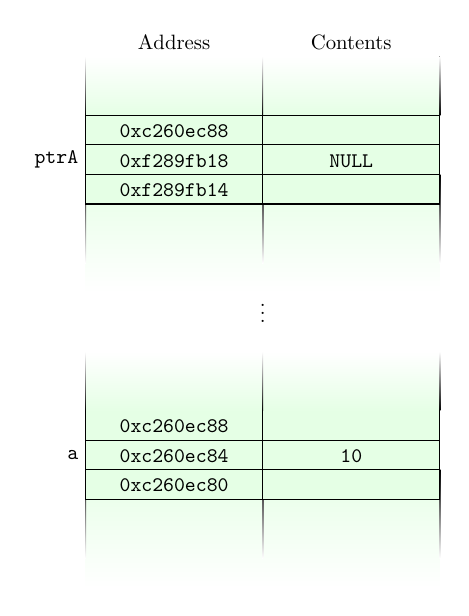
\begin{tikzpicture}[auto,scale=.75,transform shape,every node/.style={text centered}]


\path [top color=green!10!white, bottom color=white] (0,3) rectangle (6,5);
\fill [top color=black, bottom color=white] (-0.0075,3.5) rectangle (.01,5);
\fill [top color=black, bottom color=white] (2.9925,3.5) rectangle (3.01,5);
\fill [top color=black, bottom color=white] (5.9925,3.5) rectangle (6.01,5);

\draw[fill=green!10!white] (0, 4.5) rectangle (3, 5);
\node [above] (aa1) at (1.5,4.5) {\texttt{0xc260ec80}};
\draw[fill=green!10!white] (3, 4.5) rectangle (6, 5);
\node [above] (aa2) at (4.5,4.5) {~};

\draw[fill=green!10!white] (0, 5) rectangle (3, 5.5);
\node [above] (bb1) at (1.5,5) {\texttt{0xc260ec84}};
\draw[fill=green!10!white] (3, 5) rectangle (6, 5.5);
\node [above] (bb2) at (4.5,5) {\texttt{10}};
\node [left] (XX) at (0,5.25) {\texttt{a}};

\draw[fill=green!10!white] (0, 5.5) rectangle (3, 6);
\node [above] (cc1) at (1.5,5.5) {\texttt{0xc260ec88}};
\draw[fill=green!10!white] (3, 5.5) rectangle (6, 6);
\node [above] (cc2) at (4.5,5.5) {~};

%\draw [decorate,decoration={brace,amplitude=5pt},xshift=-4pt,yshift=0pt] (0, 4.5) -- (0, 6) node [text width=3cm,align=center,black,midway,xshift=-.25cm]  {\mintinline{c}{sum()} stack frame};

\path [top color=white, bottom color=green!10!white] (0,6.01) rectangle (6,7);
\fill [top color=white, bottom color=black] (-0.00725,6) rectangle (.0075,7);
\fill [top color=white, bottom color=black] (5.9925,6) rectangle (6.0075,7);
\fill [top color=white, bottom color=black] (2.9925,6) rectangle (3.0075,7);

%%%bottom

\path [top color=green!10!white, bottom color=white] (0,8) rectangle (6,10);
\fill [top color=black, bottom color=white] (-0.0075,8.5) rectangle (.01,10);
\fill [top color=black, bottom color=white] (2.9925,8.5) rectangle (3.01,10);
\fill [top color=black, bottom color=white] (5.9925,8.5) rectangle (6.01,10);

\draw[fill=green!10!white] (0, 9.5) rectangle (3, 10);
\node [above] (aa1) at (1.5,9.5) {\texttt{0xf289fb14}};
\draw[fill=green!10!white] (3, 9.5) rectangle (6, 10);
\node [above] (aa2) at (4.5,9.5) {~};

\draw[fill=green!10!white] (0, 10) rectangle (3, 10.5);
\node [above] (bb1) at (1.5,10) {\texttt{0xf289fb18}};
\node [left] (bb1) at (0,10.25) {\texttt{ptrA}};
\draw[fill=green!10!white] (3, 10) rectangle (6, 10.5);
\node [above] (bb2) at (4.5,10) {\texttt{NULL}};

\draw[fill=green!10!white] (0, 10.5) rectangle (3, 11);
\node [above] (cc1) at (1.5,10.5) {\texttt{0xc260ec88}};
\draw[fill=green!10!white] (3, 10.5) rectangle (6, 11);
\node [above] (cc2) at (4.5,10.5) {~};

%\draw [decorate,decoration={brace,amplitude=5pt},xshift=-4pt,yshift=0pt] (0, 4.5) -- (0, 6) node [text width=3cm,align=center,black,midway,xshift=-.25cm]  {\mintinline{c}{sum()} stack frame};

\path [top color=white, bottom color=green!10!white] (0,11.01) rectangle (6,12);
\fill [top color=white, bottom color=black] (-0.00725,11) rectangle (.0075,12);
\fill [top color=white, bottom color=black] (5.9925,11) rectangle (6.0075,12);
\fill [top color=white, bottom color=black] (2.9925,11) rectangle (3.0075,12);

\node (dots) at (3, 7.75) {$\vdots$};

\node[above] (x1) at (1.5,12) {Address};
\node[above] (x2) at (4.5,12) {Contents};

%\draw[fill=black] (5.75, 10.25) circle (1pt);
%\draw[blue,->] (5.75, 10.25) -- (6.5, 10.25) -- (6.5,8) -- (-1,8) -- (-1,5.25) -- (XX.west);

\end{tikzpicture}
}~~~~~~~~\subfigure[Making \mintinline{c}{ptrA} point to the variable \mintinline{c}{a}'s
memory location.  The value stored in the variable \mintinline{c}{ptrA} is a
memory address.]{

\begin{tikzpicture}[auto,scale=.75,transform shape,every node/.style={text centered}]


\path [top color=green!10!white, bottom color=white] (0,3) rectangle (6,5);
\fill [top color=black, bottom color=white] (-0.0075,3.5) rectangle (.01,5);
\fill [top color=black, bottom color=white] (2.9925,3.5) rectangle (3.01,5);
\fill [top color=black, bottom color=white] (5.9925,3.5) rectangle (6.01,5);

\draw[fill=green!10!white] (0, 4.5) rectangle (3, 5);
\node [above] (aa1) at (1.5,4.5) {\texttt{0xc260ec80}};
\draw[fill=green!10!white] (3, 4.5) rectangle (6, 5);
\node [above] (aa2) at (4.5,4.5) {~};

\draw[fill=green!10!white] (0, 5) rectangle (3, 5.5);
\node [above] (bb1) at (1.5,5) {\texttt{0xc260ec84}};
\draw[fill=green!10!white] (3, 5) rectangle (6, 5.5);
\node [above] (bb2) at (4.5,5) {\texttt{10}};
\node [left] (XX) at (0,5.25) {\texttt{a}};

\draw[fill=green!10!white] (0, 5.5) rectangle (3, 6);
\node [above] (cc1) at (1.5,5.5) {\texttt{0xc260ec88}};
\draw[fill=green!10!white] (3, 5.5) rectangle (6, 6);
\node [above] (cc2) at (4.5,5.5) {~};

%\draw [decorate,decoration={brace,amplitude=5pt},xshift=-4pt,yshift=0pt] (0, 4.5) -- (0, 6) node [text width=3cm,align=center,black,midway,xshift=-.25cm]  {\mintinline{c}{sum()} stack frame};

\path [top color=white, bottom color=green!10!white] (0,6.01) rectangle (6,7);
\fill [top color=white, bottom color=black] (-0.00725,6) rectangle (.0075,7);
\fill [top color=white, bottom color=black] (5.9925,6) rectangle (6.0075,7);
\fill [top color=white, bottom color=black] (2.9925,6) rectangle (3.0075,7);

%%%bottom

\path [top color=green!10!white, bottom color=white] (0,8) rectangle (6,10);
\fill [top color=black, bottom color=white] (-0.0075,8.5) rectangle (.01,10);
\fill [top color=black, bottom color=white] (2.9925,8.5) rectangle (3.01,10);
\fill [top color=black, bottom color=white] (5.9925,8.5) rectangle (6.01,10);

\draw[fill=green!10!white] (0, 9.5) rectangle (3, 10);
\node [above] (aa1) at (1.5,9.5) {\texttt{0xf289fb14}};
\draw[fill=green!10!white] (3, 9.5) rectangle (6, 10);
\node [above] (aa2) at (4.5,9.5) {~};

\draw[fill=green!10!white] (0, 10) rectangle (3, 10.5);
\node [above] (bb1) at (1.5,10) {\texttt{0xf289fb18}};
\node [left] (bb1) at (0,10.25) {\texttt{ptrA}};
\draw[fill=green!10!white] (3, 10) rectangle (6, 10.5);
\node [above] (bb2) at (4.5,10) {\texttt{0xc260ec84}};

\draw[fill=green!10!white] (0, 10.5) rectangle (3, 11);
\node [above] (cc1) at (1.5,10.5) {\texttt{0xc260ec88}};
\draw[fill=green!10!white] (3, 10.5) rectangle (6, 11);
\node [above] (cc2) at (4.5,10.5) {~};

%\draw [decorate,decoration={brace,amplitude=5pt},xshift=-4pt,yshift=0pt] (0, 4.5) -- (0, 6) node [text width=3cm,align=center,black,midway,xshift=-.25cm]  {\mintinline{c}{sum()} stack frame};

\path [top color=white, bottom color=green!10!white] (0,11.01) rectangle (6,12);
\fill [top color=white, bottom color=black] (-0.00725,11) rectangle (.0075,12);
\fill [top color=white, bottom color=black] (5.9925,11) rectangle (6.0075,12);
\fill [top color=white, bottom color=black] (2.9925,11) rectangle (3.0075,12);

\node (dots) at (3, 7.75) {$\vdots$};

\node[above] (x1) at (1.5,12) {Address};
\node[above] (x2) at (4.5,12) {Contents};

\draw[fill=black] (5.75, 10.25) circle (1pt);
\draw[blue,->] (5.75, 10.25) -- (6.5, 10.25) -- (6.5,8) node[below] {\mintinline{c}{ptrA = &a;}} -- (-1,8) -- (-1,5.25) -- (XX.west);

\end{tikzpicture}
}

\subfigure[Dereferencing \mintinline{c}{ptrA} and assigning a value changes
the value stored at what it \emph{points} to.]{

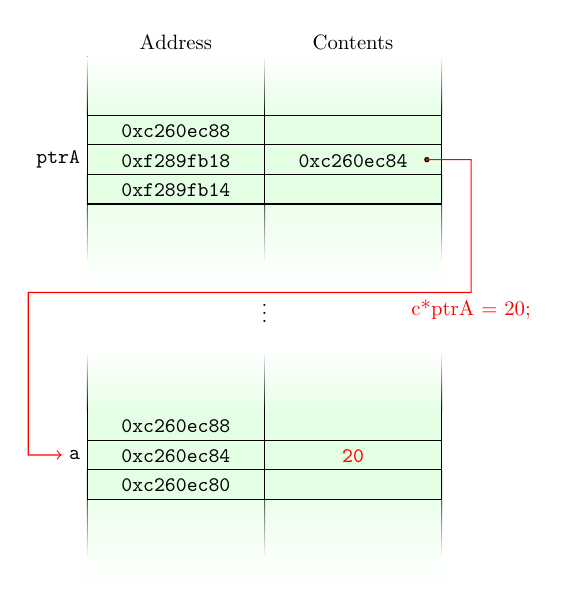
\begin{tikzpicture}[auto,scale=.75,transform shape,every node/.style={text centered}]


\path [top color=green!10!white, bottom color=white] (0,3) rectangle (6,5);
\fill [top color=black, bottom color=white] (-0.0075,3.5) rectangle (.01,5);
\fill [top color=black, bottom color=white] (2.9925,3.5) rectangle (3.01,5);
\fill [top color=black, bottom color=white] (5.9925,3.5) rectangle (6.01,5);

\draw[fill=green!10!white] (0, 4.5) rectangle (3, 5);
\node [above] (aa1) at (1.5,4.5) {\texttt{0xc260ec80}};
\draw[fill=green!10!white] (3, 4.5) rectangle (6, 5);
\node [above] (aa2) at (4.5,4.5) {~};

\draw[fill=green!10!white] (0, 5) rectangle (3, 5.5);
\node [above] (bb1) at (1.5,5) {\texttt{0xc260ec84}};
\draw[fill=green!10!white] (3, 5) rectangle (6, 5.5);
\node [above] (bb2) at (4.5,5) {\color{red}{\texttt{20}}};
\node [left] (XX) at (0,5.25) {\texttt{a}};

\draw[fill=green!10!white] (0, 5.5) rectangle (3, 6);
\node [above] (cc1) at (1.5,5.5) {\texttt{0xc260ec88}};
\draw[fill=green!10!white] (3, 5.5) rectangle (6, 6);
\node [above] (cc2) at (4.5,5.5) {~};

%\draw [decorate,decoration={brace,amplitude=5pt},xshift=-4pt,yshift=0pt] (0, 4.5) -- (0, 6) node [text width=3cm,align=center,black,midway,xshift=-.25cm]  {\mintinline{c}{sum()} stack frame};

\path [top color=white, bottom color=green!10!white] (0,6.01) rectangle (6,7);
\fill [top color=white, bottom color=black] (-0.00725,6) rectangle (.0075,7);
\fill [top color=white, bottom color=black] (5.9925,6) rectangle (6.0075,7);
\fill [top color=white, bottom color=black] (2.9925,6) rectangle (3.0075,7);

%%%bottom

\path [top color=green!10!white, bottom color=white] (0,8) rectangle (6,10);
\fill [top color=black, bottom color=white] (-0.0075,8.5) rectangle (.01,10);
\fill [top color=black, bottom color=white] (2.9925,8.5) rectangle (3.01,10);
\fill [top color=black, bottom color=white] (5.9925,8.5) rectangle (6.01,10);

\draw[fill=green!10!white] (0, 9.5) rectangle (3, 10);
\node [above] (aa1) at (1.5,9.5) {\texttt{0xf289fb14}};
\draw[fill=green!10!white] (3, 9.5) rectangle (6, 10);
\node [above] (aa2) at (4.5,9.5) {~};

\draw[fill=green!10!white] (0, 10) rectangle (3, 10.5);
\node [above] (bb1) at (1.5,10) {\texttt{0xf289fb18}};
\node [left] (bb1) at (0,10.25) {\texttt{ptrA}};
\draw[fill=green!10!white] (3, 10) rectangle (6, 10.5);
\node [above] (bb2) at (4.5,10) {\texttt{0xc260ec84}};

\draw[fill=green!10!white] (0, 10.5) rectangle (3, 11);
\node [above] (cc1) at (1.5,10.5) {\texttt{0xc260ec88}};
\draw[fill=green!10!white] (3, 10.5) rectangle (6, 11);
\node [above] (cc2) at (4.5,10.5) {~};

%\draw [decorate,decoration={brace,amplitude=5pt},xshift=-4pt,yshift=0pt] (0, 4.5) -- (0, 6) node [text width=3cm,align=center,black,midway,xshift=-.25cm]  {\mintinline{c}{sum()} stack frame};

\path [top color=white, bottom color=green!10!white] (0,11.01) rectangle (6,12);
\fill [top color=white, bottom color=black] (-0.00725,11) rectangle (.0075,12);
\fill [top color=white, bottom color=black] (5.9925,11) rectangle (6.0075,12);
\fill [top color=white, bottom color=black] (2.9925,11) rectangle (3.0075,12);

\node (dots) at (3, 7.75) {$\vdots$};

\node[above] (x1) at (1.5,12) {Address};
\node[above] (x2) at (4.5,12) {Contents};

\draw[fill=red] (5.75, 10.25) circle (1pt);
\draw[red,->] (5.75, 10.25) -- (6.5, 10.25) -- (6.5,8) node[below] {\mintinline{c}{*ptrA = 20;}} -- (-1,8) -- (-1,5.25) -- (XX.west);

\end{tikzpicture}
}


\caption[Pointer Operations]{Pointer Operations.  Pointers can be made to point to
other variable's memory locations.  You can manipulate/access values of variables 
via their pointers using dereferencing.}
\label{figure:cPointers}

\end{figure}




%\end{document}


\subsection{Passing By Reference}
\index{pass by reference}

Now that we have the ability to reference a memory location 
using pointers, we can write functions that pass variables by 
reference.  To do so, we use the same asterisk syntax used
with pointer variables.

\begin{minted}{c}
//prototypes
/**
 * This function sums the first two variables (passed by
 * value) and places the result into the third variable 
 * (passed by reference).
 */
void sum(int a, int b, int *c);

/**
 * This function swaps the values stored in the
 * two variables passed by reference.
 */
void swap(int *a, int *b);
\end{minted}

In the function definitions, we can use the dereferencing
operator to access or modify the value stored in the
variable pointed to by the pointer.  

\begin{minted}{c}
void sum(int a, int b, int *c) {
  int x = a + b;
  *c = x;
  return;
}

void swap(int *a, int *b) {
  int temp = *a;
  *a = *b;
  *b = temp;
  return;
}
\end{minted}

To invoke these functions, we need to pass pointers to 
the functions appropriately.  We could do this by
creating pointer variables or using the referencing operator
directly.

\begin{minted}{c}
int x = 10;
int y = 20;
int c;
int *ptrC = &c;
sum(x, y, ptrC);
//at this point c contains the value 30

swap(&x, &y);
//at this point, the values in x and y have been swapped
// x contains 20 and y contains 10
\end{minted}

This should look familiar.  We saw this same syntax when
we used \mintinline{c}{scanf()} to read input from the standard
input.  We needed to place an ampersand in front of each
variable in order to pass the variable by reference so that
\mintinline{c}{scanf()} could place the results into the respective
memory locations.  If the variables had been passed by 
value, then \mintinline{c}{scanf()} would not have been able
to manipulate their values.

You can also specify functions to \emph{return} pointers
which we discuss in detail in Chapter \ref{chapter:c:arrays}.

\subsection{Function Pointers}

Functions are just pieces of code that reside somewhere in 
memory just as variables do.  Since we can create pointers
that point to variables, it makes sense to be able to create
variables that point to functions too!  These are referred to
as \emph{function pointers}.  

The syntax for declaring function pointers is similar to variable
pointers.  However, since a function's signature involves a
return type and parameter list, these need to be specified.
For example, suppose we wanted to create a function pointer
that could point to the math library's \mintinline{c}{sqrt()} function
which takes a single \mintinline{c}{double} parameter and
returns a \mintinline{c}{double} value.  

\mintinline{c}{double (*ptrToSqrt)(double) = NULL;}

The above line creates a function pointer that can point to
any function that takes a single \mintinline{c}{double} parameter
and returns a \mintinline{c}{double} value.  As is good practice,
we've initialized it to point to \mintinline{c}{NULL}.  The function
pointer itself is named \mintinline{c}{ptrToSqrt}.  To make it
point to the \mintinline{c}{sqrt()} function we can use the following
syntax.

\mintinline{c}{ptrToSqrt = sqrt;}

This is because a function's identifier acts as a pointer as well!
Once we have a pointer to a function, we can invoke the function
via its pointer as we would any other function call.

\mintinline{c}{double x = ptrToSqrt(2.0);}

Some more examples:

\begin{minted}{c}
//this pointer can point any function that takes
//three arguments: an int, double, and a char
//and returns an int value
int (*ptrToFunc)(int, double, char)= NULL;

double x;
double (*ptr)(double) = NULL;
//we can make it point to sqrt:
ptr = sqrt;
x = ptr(2.0); //x contains 1.4142...
//or we can make it point to fabs
ptr = fabs;
x = ptr(-10.5); //x contains 10.5
\end{minted}

You generally want to create and use function pointers when
passing and returning functions as arguments to other
functions as callbacks.  We discuss this in further detail
in Chapter \ref{chapter:c:searchingSorting}.

\section{Examples}

\subsection{Generalized Rounding}

Recall that the standard math library provides a \mintinline{c}{round()}
function that rounds a number to the nearest whole number.  We've
had need to round to cents as well.  We now have the ability to write
a function to do this for us.  Before we do, however, let's think more
generally.  What if we wanted to round to the nearest tenth?  Or
what if we wanted to round to the nearest 10s or 100s place?  Let's
write a general purpose rounding function that allows us to specify
\emph{which} decimal place to round to.  

The most natural input values would be to specify the place using
an integer exponent.  That is, if we wanted to round to the nearest
tenth, then we would pass it $-1$ as $0.1 = 10^{-1}$, $-2$ if we wanted
to round to the nearest 100th, etc.  In the other direction, passing in 0
would correspond to the usual round function, 1 to the nearest 10s spot, 
and so on.  Moreover, we could demonstrate good code reuse (as well as 
\index{procedural abstraction} procedural
abstraction) by \emph{scaling} the input value and reusing the functionality
already provided in the math library's \mintinline{c}{round()} function.  We
could further define a \mintinline{c}{roundToCents()} function that used 
our generalized round function.

Let's also think about organization.  We could place the prototypes into
a \mintinline{text}{round.h} header file and the corresponding definitions
in a \mintinline{text}{round.c} source file.  The contents of these two
files are presented here:

\begin{minted}{c}
/**
 * Rounds to the nearest digit specified by the place
 * argument.  In particular to the (10^place)-th digit
 */
double roundToPlace(double x, int place);

/**
 * Rounds to the nearest cent
 */
double roundToCents(double x);
\end{minted}

\begin{minted}{c}
#include<math.h>
#include "round.h"

double roundToPlace(double x, int place) {
  double scale = pow(10, -place);
  double rounded = round(x * scale) / scale;
  return rounded;
}

double roundToCents(double x) {
  return roundToPlace(x, -2);
}
\end{minted}

Observe that neither of these files contains a \mintinline{c}{main()}
function.  By themselves they would not be able to be compiled
into an executable program.  We've essentially built a small 
\emph{library} of rounding functions.  We could compile them though
into a binary \emph{object} file using gcc (something like 
\mintinline{text}{gcc -c round.c}).  We could then link into the object
file when compiling an executable program that uses these functions.

\subsection{Quadratic Roots}
\label{subsection:c:quadraticRoots}

Another advantage of passing variables by reference is that we
can ``return'' multiple values with one function call.  Functions
are limited in that they can only return at most one value.  But
if we pass multiple parameters by reference, the function can
manipulate the contents of them, thereby communicating (though
not strictly returning) multiple values.  

Consider again the problem of computing the roots of a quadratic
equation, 
  $$ax^2 + bx + c = 0$$
using the quadratic formula,
 $$\frac{-b \pm \sqrt{b^2 - 4ac}}{2a}$$
Since there are two roots, we may have to write two functions, 
one for the ``plus'' root and one for the ``minus'' root both of 
which take the coefficients, $a, b, c$ as arguments.  However,
if we wrote a single function that took the coefficients as parameters
by value as well as two other parameters by reference, we could
compute \emph{both} root values and place each one in two pass 
by reference variables.

\begin{minted}{c}
void quadraticRoots(double a, double b, double c, 
                    double *root1, double *root2) {
  double discriminant = sqrt(b*b - 4*a*c);
  *root1 = (-b + discriminant) / (2*a);
  *root2 = (-b - discriminant) / (2*a);
  return;
}
\end{minted}

By using pass by reference variables, we avoid multiple functions.
We also note that the return value in this case is unused since
we are ``returning'' the root values in the two pass by reference
variables.  This frees up the return value to be used to communicate
\emph{errors} to the calling function.  Recall that there could
be several ``bad'' inputs to this function.  The roots could be complex
values, the coefficient $a$ could be zero, etc.  And now that we
are dealing with pointers, the pointers could be invalid (point to
\mintinline{c}{NULL}).  In the next chapter, we examine how we
can use the return value to communicate different errors to the
calling function, letting it \emph{handle} those errors.







